\section{Figure Rendering}

\subsection{3D Plots}

\begin{figure}[h]
    \centering
    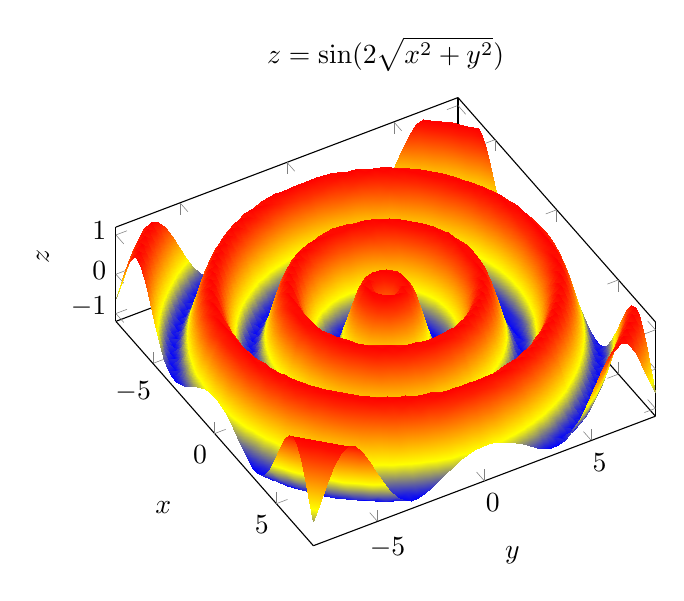
\begin{tikzpicture}
    \begin{axis}[
        title={$z = \sin(2\sqrt{x^2 + y^2})$},
        xlabel={$x$},
        ylabel={$y$},
        zlabel={$z$},
        domain=-8:8,
        y domain=-8:8,
        view={60}{70},
        samples=50
    ]
    \addplot3[
        surf,
        shader=interp,
    ]
    {sin(deg(2*sqrt(x^2 + y^2)))};
    \end{axis}
    \end{tikzpicture}
    \caption{3D plot of $z = \sin(2\sqrt{x^2 + y^2})$}
\end{figure}